\graphicspath{ {./chapters/Side_Channels} }

\section{What is a Side-Channel?}

\section{Fine-Grained Analysis of Physically Observable SC}
  \subsection{Frequency-Domain Analysis of EM Side-Channels}
    Remember that periodic activities have a spectral component at $f_1 = 1/t_1$ where $t_1$ is the time to complete the periodic activity.
    Tracking the code over time it will present with the spectral component of the current task.
    When another task is performed the spectral components will change which can be seen in the side channel and allows tracking of program flow.

    Remember that a clock is a periodic activity on which the program execution can be modulated.
    This allows us to observe the spectrum at higher frequencies where there is less environmental noise.

    Also remember that malware can be detected using the spectral components of the executed program.
    For example if malicious code is inserted during the loop the spectral component decrease in frequency compared to the expected EM frequency.
    However, if code is deleted during a loop the spectral component will increase and also be detectable.
    Finally, if code is inserted between loops it will be seen in the break between where the loops are expected to transition.

    So this raises the question: how do we identify repetitive structures in the spectrum?

    \subsubsection{HDBSCAN}

      One powerful tool to automate the location of repetitive structures in the spectrum is known as HDBSCAN.

      \begin{defbox}[HDBSCAN]
        Hierarchical density-based spatial clustering of applications with noise
      \end{defbox}

      HDBSCAN works by:
      \begin{enumerate}
        \item Transform the space according to the density
        \item Builds the minimum spanning tree of the distance weighted graphic
        \item Constructs a cluster hierarchy of connected components
        \item Condenses the cluster hierarchy based on the minimum cluster size
        \item Extracted the stable clusters from the condensed tree
      \end{enumerate}

      Once the clusters are identified peaks may be detected.
      The peaks correspond to the harmonics of the spectral component.
      These peaks are then used to check when the spectrum is in this loop and determine if the loop has been altered or left.
      If any of the harmonic peaks is different it is likely the loop has been altered or it is a different loop.

    \subsection{Dimension Reduction}

      An alternative to HDBSCAN is two-phase-dimension-reduction.
      As the name indicates two-phase-dimension-reduction works in two stages. 

      The first phase averages the magnitudes of the short-time fourier (STFT) transform using \autoref{eq:tpdr_phase_1}.
      This enables a the noise and the number of samples to be reduced.
      Note that in this equation $X_l[k]$ is the STFT spectrogram's $k^{th}$ component and $N_R$ is the number of samples which are averaged together.

      \begin{equation}
        \label{eq:tpdr_phase_1}
        x_i[k] = \frac{1}{N_R} \sum_{l = 1}^{N_R} \vert X_l[k] \vert
      \end{equation}

      Phase two applies principal component analysis (PCA) to the result from phase one represented as a matrix (see \autoref{eq:tpdr_phase_2_matrix}).
      In the matrix $m$ represents the total number of measurements.
      $\hat{x_i}[k] = 10 \log_{10}(|x_i[k]|^2)$ is used in order to filter out the linear effects of the STFT.
      Thus each column in the matrix represents an averaged frequency component of the signal in the dB-domain.

      \begin{equation}
        \label{eq:tpdr_phase_2_matrix}
        \begin{bmatrix}
          \cdots & \hat{x_1} & \cdots \\
          \cdots & \hat{x_2} & \cdots \\
                 & \vdots    &        \\
          \cdots & \hat{x_m} & \cdots
        \end{bmatrix}
      \end{equation}

      The first part of the PCA is then to find the model for the system.
      This is done through singular value decomposition (SVD).
      SVD provides a method of creating a series of orthonormal (un-correlated linear relationships) which can be used to reduce a 
        large variable space into a significantly smaller variable space (i.e. can reduce the number of variables needed to represent a vector).

      This is then used to create a smaller dimension array which can be easily analyzed using the k-th nearest neighbor algorithm (k-NN).

      Using PCA provides several benefits.
      The first and foremost is that different operations use various frequency components, 
        but tracking all frequency components can require a high-level of overhead.
      However, frequency components and corresponding  thresholds must be conservatively set in order to ensure
        data size reduction without loss of variation between classes.

      \begin{algobox}[Two-Phase Dimension Reduction]
        \label{algo:tpdr}
        \begin{enumerate}
          \item Measure Emanated Signal for T seconds
          \item Reduce dimension using Phase One technique to get $X$
          \item Apply Phase 2 to $X$ to generate mode
          \item Collect testing signal $z$ and apply Phase One to get $\hat{z}$
          \item Project the test signal $\mathcal{Z} = \hat{z} V_K \sigma_K^{-1}$
          \item Apply k-NN algorithm to approximate the status of the device
        \end{enumerate}
      \end{algobox}

  \subsection{Detecting Malware Using Frequency-Domain}

    One potential use for frequency-domain side-channels is to detect malware.
    This can be done by looking for anomalies in the spectrogram generated during program run.
    In order to easily find these it is important to understand the various spectrographic shapes which a loop can take.

    Generally speaking there are three types of loop: fixed, control-flow, and nested.
    Each loop has a distinct spectral signature.
    Fixed loops are extremely stable as they perform the exact same operations repeatedly,
      thus their spectral signature is a single large peak.
    Control-flow loops on the other hand have internal branches which depend on the input to the loop.
    This gives these loops a multi-peak signature, with the different peaks representing the different paths through the loop.
    Finally nested loops contain many sub-loops. 
    If these loops are adequately long they may be detected as multi-peak spectrums, but ordinarily they present as broad spectrum peaks.

    In order to detect malware injection statistical tests are used. 
    Due to the non-gaussian nature of the spectrograms it is necessary to use non-parametric tests.
    One such option is the K-S test which is sensitive to any difference between two groups of distribution.

    Using a statistical test like this it is necessary to weight the tradeoff between detection latency and accuracy.
    On the one-hand we want to determine if malicious code is running on the processor as quickly as possible.
    However, we also do not want to flag good code or ignore malicious code.
    Thus we must increase the number of samples until the false rejection rate drops to a sufficient level.

    How long this takes can depend heavily on the type of loop that is intended to be run.
    In general the fixed loop is the easiest to notice a change in due to its sharp singular feature,
     which is easily distinguished from other features.
    On the other end of the spectrum is the nested loop.
    Because of its broad peak many more samples are needed to distinguish generalized noise from a malicious attack.

  \subsection{Time-Domain Analysis of EM Side-Channels}
    While frequency-domain analysis is simple and extremely useful for determining broad information about the running program,
      it lacks the precision to dive deep into the inner workings of the program being observed.
    This is where Time-Domain analysis comes in.
    The time-domain provides a significantly finer grained analysis than frequency domain, which enables it to be used for
      program tracking from control flow down to individual instructions.
    
    In order to achieve a clear signal for use in this sort of analysis the EM emanations must be extracted.
    This is done through amplitude demodulation.
    Because the clock frequency is the strongest signal in the circuit its effects must be filtered out.
    To do so the EM signal is demodulated with respect to the clock frequency using \autoref{eq:amp_demodulation}

    \begin{equation}
      \label{eq:amp_demodulation}
      x(t) = | r(t) \times e^{j2\pi f_c t} |
    \end{equation}

    The first step towards using time-domain analysis is to determine what the expected emanations will look like.
    This is often done by running semi-random data through a program or part of program.
    If this is done enough times for each execution path an expected waveform which contains distinguishable 
      characteristics can be determined from an average of traces.
    This allows a single trace, or set of traces averaged out, to be compared against the expected behavior for the different
      execution paths.
    By finding the correlation between the target signal and the expected signal the best and most probable match can be found.

    This is a simple method, but can we do better?

    \subsubsection{Machine-Learning Techniques for EM Side-Channel Tracking}
      Machine learning techniques can be used to for automated fine-grain analysis of code execution.
      These techniques are not without issue though as some can lead to high computational explosion as the 
        code-base increases in size.
      Machine learning is performed by first finding a set of training inputs which cover the entire flow-control space.
      These are then used on a known good training system to collect a series of waveforms which are used to 
        train the ML model.
      A waveform can then be collected from a fielded system and analyzed in order to determine the flow 
        path and the presence of any malicious code.

      The program structure can be further leveraged to improve these techniques.
      By noting that some blocks of code will always execute together these can be used as singular references.
      It is also useful to note that these blocks will always process in a limited set of order 
        (i.e. that not all code blocks can execute after any other code block).
      This allows an input wave form to be divided and analyzed using correlation to these subsets.
      A greedy tree-search can then be used to piece together the full execution path of the given wave form.

      However, this tree search and correlation approach is limited in several key ways.
      Firstly it is difficult to scale to larger programs due to the infeasibility of determining all of the flow
        control paths and the additional memory and computational overhead of comparing a growing number of reference blocks.
      Additionally, the greedy tree-search is rather inefficient.

      One way to improve this is to perform the path prediction with a hidden Markov model.
      This allows the algorithm to use additional states between within the blocks of code which have been identified.
      However, hidden Markov models still fail to scale well and rely on several key assumptions about the underlying program.
      Such assumptions includes statistically stationary transition probabilities and the presence of hidden information.

    \subsubsection{Speech Recognition Techniques for EM Side-Channel Analysis}
      An alternative to the relatively simple ML techniques previously discussed is the use of speech recognition 
        techniques of the processing of a wave form.
      This option is believed to better manage the computational complexity of larger problems.
      The speech recognition used for EM analysis is based on forming a reduced dictionary and then using the dictionary 
        to classify the signal being monitored.

      In order to construct the original dictionary the EM signal is collected from a known-good source.
      This signal is then split into many overlapping short-duration fixed-length windows. 
      Each windows is recorded as a dictionary entry (or a word in speech).
      A clustering technique can then be used to reduce the dictionary.
      One strong clustering candidate is threshold-based clustering which relies on continually growing centroids
        which aggregate surrounding dictionary entries into strong approximation models.
      
      Once the reduced dictionary is constructed an EM signal is captured for analysis.
      Then each window in the EM signal is replaced by its best mach dictionary entry.
      If the dictionary entries were tagged with known code segments this allows for an approximate flow-control to be determined.
      Alternatively, if the desire is simply to monitor for anomalies then the error between the signal and the 
        substituted entries can be used with a simple threshold to determine whether the variance falls into normal operating
        conditions.
      Increasing the complexity slightly to use a moving average filter for the anomaly threshold has been shown to 
        substantially decrease the false positive rate.

      Speech recognition techniques have excellent performance for malware detection without requiring a malware signature.
      Additionally, if malware detection is the only goal then the source code and control-flow graph are not required.
      However, as the program run-time increases the dictionary size may grow substantially.
      The speech recognition technique is also computationally inefficient during classification.

    \subsubsection{Neural Network Techniques for EM Side-Channel Analysis}
      Another method for fine-grained EM analysis is the use of a neural network.
      Many architectures of NN may be used for this technique. 
      Multilayer perceptrons (MLP) have shown strong results in experiments.
      The neural network is tasked to find the expected amplitude of an EM signal at any given instance.
      In cases where real-time monitoring is not required a non-causal model may be used which significantly increases
        the efficacy of the method as it allows access to data before and after the instant being predicted.

      While NNs require a longer training period than the other methods previously discussed they have some 
        distinct advantages.
      A NN evaluation is constant time for a single evaluation which allows linear time evaluation of signals.
      Additionally, because the NN is a fixed size it has a constant memory complexity regardless of program size.

\section{Covert-Channels}
  Covert-channels are a form of communication which is designed to not be obviously visible to the system.
  This often involves directly leveraging side-channels such as EM emanations in order to turn a processor 
    into an RF transmitter.
  For example if a pair of loops can be found with different power characteristics they can be looped in a known
    way and create an amplitude modulated signal.
  Another style of covert channel could be to repeat specific instructions in order to enhance signal strength
    and increase the ease of detecting that instruction.
  Increasingly popular is the use of computer power management states. 
  These have the benefit of being easily detectable, but tend to be slower than other alternatives.

  \subsection{Example Covert Channel}
    Here we demonstrate an example covert channel based on the idea of power states.
    Modern computers use demand based switching techniques to reduce power consumption when not under heavy load.
    These come in two types: performance states and processor states.
    Performance states refer to the current state of an active core, generally increasing the clock frequency
      when under heavy load and decreasing it when the processor has enough overhead to handle the task with ease.
    Processor states on the other hand denote whether a processor is active or not. 
    When a processor is parked (not active) it receives significantly lower currents and in some cases may be 
      de-clocked entirely.

    These states very clearly impact the emissions from the processor.
    However, they can impact more than the processor.
    When a CPU core is idle it may tell the voltage regulator module (VRM) to reduce the voltage level to the core.
    Because of the way modern voltage regulators operate this will significantly decrease the emissions from the device.

    We can leverage these power states using a code which alternates between power states based on the bits we desire 
      to send as shown in \autoref{algo:example_covert_channel}.

    \begin{algobox}
      \label{algo:example_covert_channel}
      \lstinputlisting[
        language=C, 
        numbers=left,
        xleftmargin=20pt
      ]{./chapters/Side_Channels/example_covert_channel.c}
    \end{algobox}

    This algorithm works by shifting the power state from active to sleep for a $1$, but leaving it asleep for $0$ bits.
    Thus a RF receiver can see significant shifts in the magnitude of the frequency components.
    
    An approach such as this is not without issues though.
    Consider the case where the program is interrupted by another activity such as the OS.
    This will cause the CPU to become active before returning control to the covert program.
    Additionally, in modern processors the power state of the CPU may not be strictly controlled by a single program
      as there are likely to be other programs which desire to run during the sleep time, or which run on the same
      physical processor using simultaneous multi-threading.

  \subsection{Modeling Covert Channels}
    Now that we've seen how to create a covert channel, we want to know how to model them.

    First consider how the analog signals are created.
    The current in modern processors occurs from bit-flips through transistors.
    However, modeling every transistor in a system is infeasible and unnecessary.
    Instead we find a corelation between the emissions and the processor's operating condition.
    Starting with a simple pipeline it has been shown that emanations vary depending on the state of the pipeline.

    So it's simple then?
    Unfortunately not more needs to be done than just finding the power required for any given pipeline state.
    If we were to use a rectangular approximation of the signal with the power of any given state at the clock cycle
      we would get close, but still stray from the true output.
    As we see in \autoref{fig:modeling_covert_channels} a rectangular approximation is correct at the initial peak,
      but it quickly strays from the true signal.

    \begin{figure}[ht]
      \label{fig:modeling_covert_channels}
      \centering
      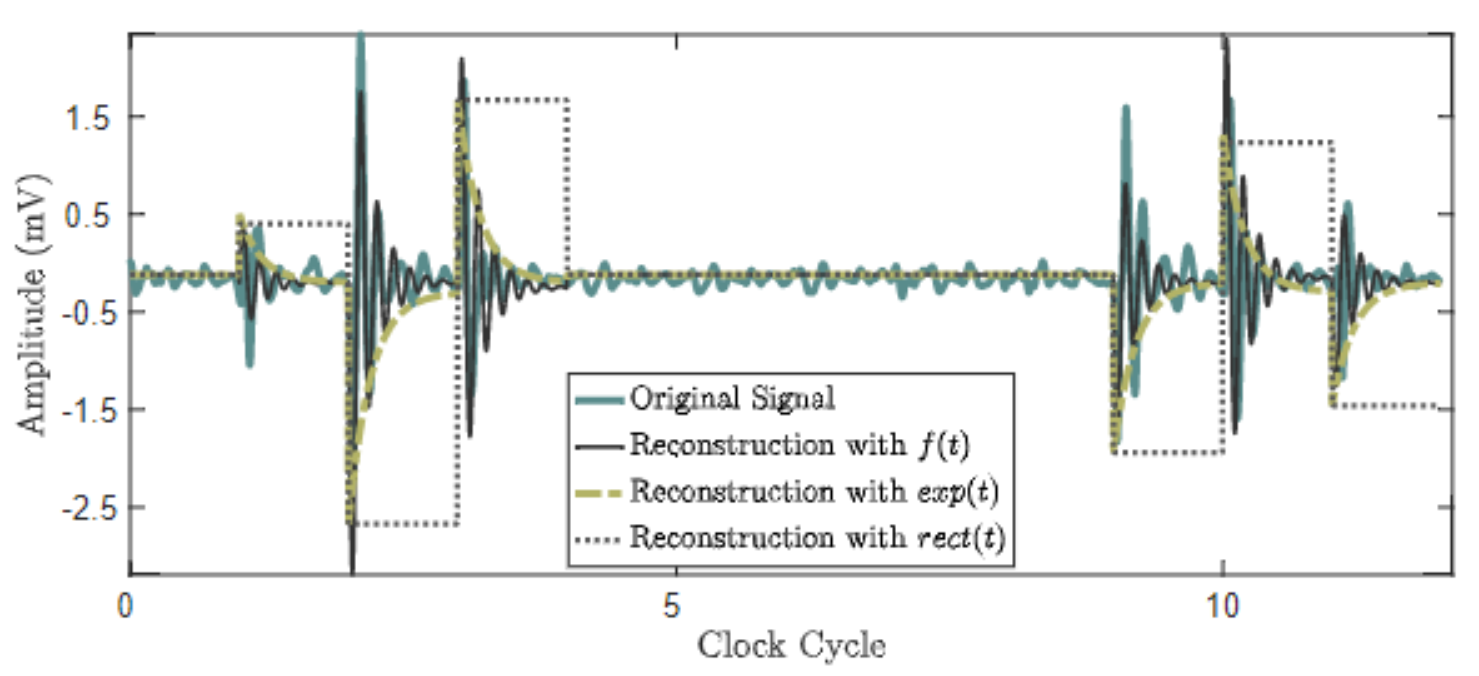
\includegraphics[width=\linewidth]{modeling_covert_channels.PNG}
      \caption{Different Covert Channel Models}
    \end{figure}

    Intuitively the next option is model with a exponential curve.
    Again we run into a problem.
    While this is closer it misses the inherent oscillation which occurs as the signal ripples through the combinatorial circuits.
    Thus we must use a more complex model which includes some form of oscillation.
    The full final signal can be represented using:

    \begin{equation}
      \label{eq:covert_channel_model}
      y(t) = \sum_{n = 1}^{\infty} x[n] \sin \left(\frac{2\pi (t-nT)}{T_0}\right) e^{-\theta (t-nT)} u(t-nT)
    \end{equation}

    Where $x[n]$ is the initial power of the pipeline state and $u(t)$ is the unit step function.

    $x[n]$ is found experimentally, but it must consider the entire state of the pipeline not just a single stage.
    However, this is known to be an aggregation of each individual stage so it can be found without an exponential search.

    This model works great for pipeline, however we are missing some things.
    Namely we are missing micro-architectural events.
    Cache misses, branch predictions, and pipeline stalls are all going to play some substantial role on the covert channel.
    Thus any fully featured model ought to account for them.

\section{Fault Injection Attacks}

  \subsection{Types of Fault}

    \subsubsection{Fault Effects}

    \subsubsection{Fault Methods}

  \subsection{}

\section{Backscattering Side-Channels}